\section{System Design}

\subsection{System Architectures}

  The system contains two different type of databases. The first databases \textbf{PlayerDB}
  combines with \textbf{TrustedDB} and \textbf{UntrustedDB} where
  presistent the player inputs whether the overall result is reliable or not. 
  A reliable player shall pass the system \textbf{Player Rating Model}. 
  Once the task result from new player is reliable, then the system will
  reuse the player input into our \textbf{Disaster Evalutation Model} and presistent it in the second
  database \textbf{ResultDB}. Stakeholder make querys to this monitoring database. 
  Figure \ref{fig:arch} illustrate the overall disaster system design.

    \begin{figure}[htp]
    \centering
    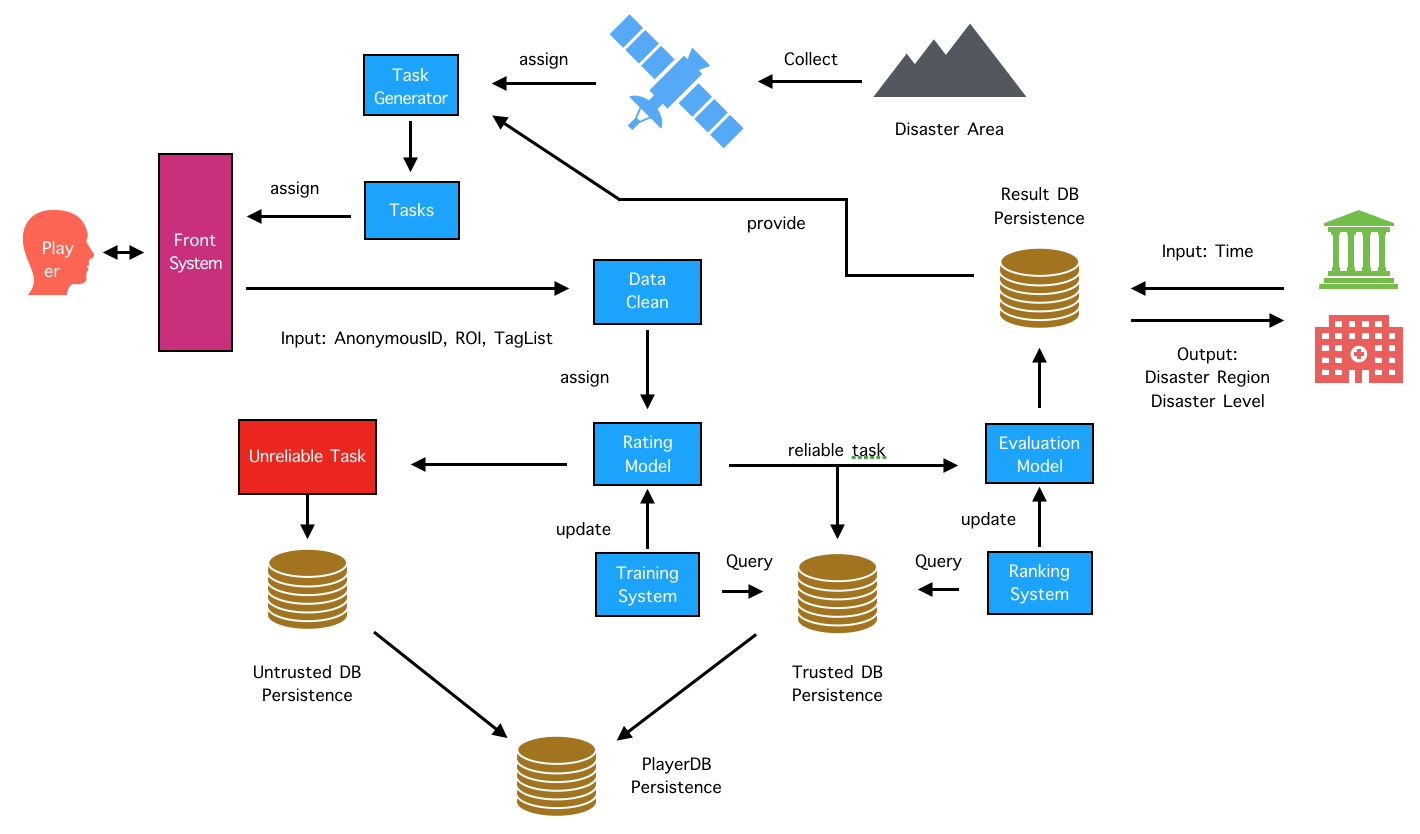
\includegraphics[width=\textwidth]{figures/system2}
    \caption{System Design Overview}
    \label{fig:arch}
    \end{figure}

  The most important issue of this human computation system is to solve weather the player\'s input
  is trustable or not. To solve this problem, we designed a \textbf{Task Generator} that combines 
  trusted results and seperate new satellite images to players. 

\subsection{System Components}

\subsubsection{Database Fields}

  For the convinience of model discusstion, we describe the system database PlayerDB Fields as follows:
and also with the fields of database ResultDB:

\noindent\begin{minipage}{.45\textwidth}
\begin{lstlisting}[
    caption={Player Database Fields},
    label={lst:trustdb}
]
[
 {
  "anonymous_id": number,
  "reliable": boolean,
  "trust_value": number
  "tasks": [
   {
    "image": image_path,
    "at_time": time, 
    "ROI": [
     {
      "latitude": number,
      "longitude": number,
      "tags": [tag1, tag2, ...]
     }, ...
    ]
   }
  ]
 }, ...
]
\end{lstlisting}
\end{minipage}\hfill
\begin{minipage}{.45\textwidth}
\begin{lstlisting}[
  caption={Results Database Fields},
  label={lst:resultdb}
]
[
 {
  "area_id": number,
  "disaster_level": number,
  "history": [
   {
    "at_time": time,
    "image": image_path,
    "ROI": [
     {
      "latitude": number,
      "longitude": number,
      "tags": [tag1, tag2, ...]
    }
   ]
  }, 
  ...
 ]
}, ...
]
\end{lstlisting}
\end{minipage}

Region of Interests (ROI)

\subsubsection{Player Task Generator}

    The \textbf{Player Task Generator (PTG)} combines images from satellite and ResultDB. 
    In the first step, as we discussed before, to solve the imformation leakage problem,
    PTG shall split a monitoring region into $m\times n$ small pieces of images, and also assign a 
    unique \textbf{areaID} for each pieces, i.e. $(\text{areaID}, \text{time})$ 
    specifice a unique image for user tasks. 

    The second generate step is to retrieve tagged images from \textbf{ResultDB}. Then combine
    all images as a user task assign to a new upcomming player. Each user task contains 
    half of untagged images and half of tagged images.

    In short, The Data Model (only ouput here) for PTG is:

    \[
    \{(\text{areaID}_1, \text{time}_1), ..., (\text{areaID}_n, \text{time}_n)\}
    \]

    with $\text{areaID}_1$ to $\text{areaID}_{\floor{n}}$ are from satellite and 
    $\text{areaID}_{\floor{n}+1}$ to $\text{areaID}_{n}$ are from \textbf{ResultDB}.

\subsubsection{Player Rating Model}

  This subsection describes the Player Rating Model inside our Disaster Monitroing system.
  PageRank was first proposed by Lary Page \cite{page1999pagerank}. It\'s commonly used for 
  expressing the stability of physical systems and the relative importance, so-called centralities, 
  of the nodes of a network. We transfer the basic idea of PageRank and use eigenvalue
  as a \textbf{Trust Value (TV)} for each players.

  Considering a partial fully connected directed graph betwen players. 
  Each player is a node of the Player Rating Graph (PRG) as illustrate in figure \ref{fig:graph}.

  \begin{figure}[htp]
  \centering
  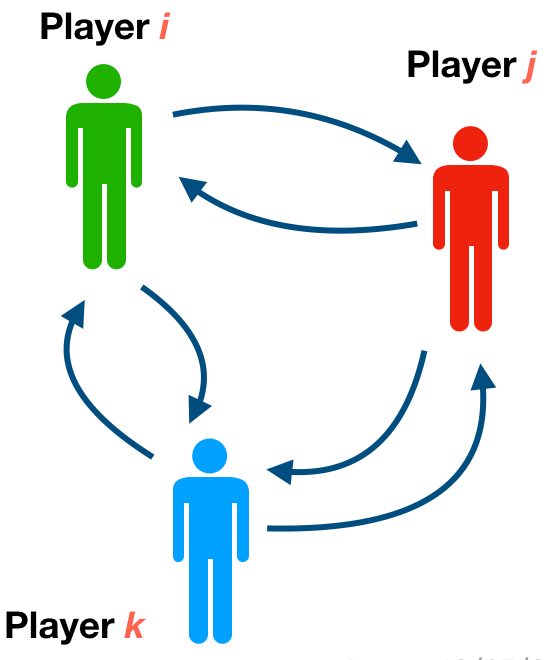
\includegraphics[width=4cm]{figures/graph}
  \caption{Player Rating Model}
  \label{fig:graph}
  \end{figure}
  
  To define the edge weight, accroding to the database feild design of a player, each player
  output ROIs for each task region of a player task, and each ROI contains a tags list, thus, 
  one can use three festures $(\text{ROI}, \text{tags}, TV)$.


  \begin{definition}
  The weight from player $i$ to player $j$ can be formalized as follows:

  \begin{equation}
  w_{ij} = 
    \sum_{\text{ROI}\in\text{ROIs}}{\text{TV}_i \times
      \frac{\text{ROI}_i\cap\text{ROI}_j}{\text{ROI}_i}
      \frac{Cov(\text{tags}_i, \text{tags}_j; v)}
          {Cov(\text{tags}_i, \text{tags}_i; v)Cov(\text{tags}_j, \text{tags}_j; v)}
    }
  \end{equation}

  where 
  
  \begin{itemize}
    \item $TV_i$ is the trust value of player $i$;
    \item $\text{ROI}_i$ is the selected ROI from player $i$;
    \item $\text{tags}_i$ is the tags from player $i$;
    \item $Cov(x, y; v)$ is the weighted covariance of $x$ and $y$ via $v$;
    \item $v$ is the weight vector of all tags.
  \end{itemize}
  \end{definition}

  This definition of  can represents the score from $i$ to $j$
  
  \[
  (\text{anonymous\_id}, \text{image}, \text{event\_time}, \text{ROI}, \text{tag\_list})
  \]

  Model output: 
  
  \[
  (\text{anonymous\_id}, \text{trust\_value})
  \]

    Note that:

    \begin{itemize}
      \item $(anonymous\_id, image, event\_time, ROI)$ is the primary key of the input vector;
      \item A player can generate multiple vectors to rating system even for same image;
      \item The event\_time is the capture time of the satellite image.
    \end{itemize}

    \begin{figure}[htp]
    \centering
    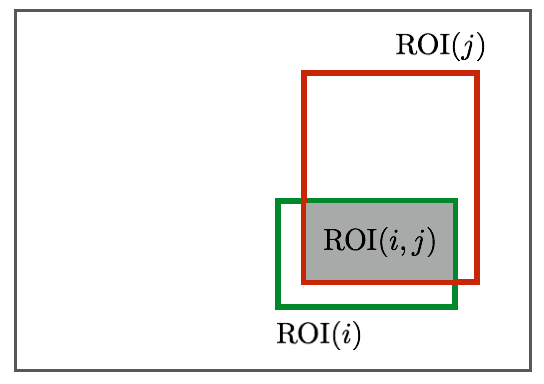
\includegraphics[width=4cm]{figures/weight-define}
    \caption{Weight Definition Visualization}
    \label{fig:roiweight}
    \end{figure}

    For a certain image $img$ at time $t$, Rating: player $i$ $\rightarrow$ player $j$:

    \[
    w_{ij}=\sum_{\text{ROI}\in \text{ROIs}}\frac{\text{ROI}(i,j)}{\text{ROI}(i)} \times \frac{Cov(\text{tags}(i), \text{tags}(j))}{\text{var}(\text{tags}(i))\text{var}(\text{tags}(j))} \geq 0
    \]

    Normalized Adjacency Matrix:

    \[
    A = (\frac{w_{ij}}{\sum_{j}{w_{ij}}})
    \]

    
    \begin{theorem}
    A is \textbf{irreducible, real, non-negative, column-stochastic, and diagonal element being positive.}
    \end{theorem}

    \begin{proof}
    blablabla
    \end{proof}

    then eigenvalue of A is the player trust value. When a new player tagging task need to be rated,

    \begin{itemize}
      \item which means we need introduce a new node to the graph
      \item need calculate the trust value of new graph
      \item let $t’$ is the trust value of new player
      \item if $t’ >= \text{mean}(\text{old\_eigenvalues})$, then it is a reliable player, otherwise drop it.
    \end{itemize}

  \subsubsection{Disaster Evaluation Model}

    System like ESP, ARTigo has proved that human inputs are valuable and useful. That\'s why we decide to let user input
    their own tags.

    Query input:

    \[
    (\text{time}) or (\text{area\_id})/(\text{area\_id}, \text{time})
    \]

    Model output:

    \[
    (\text{area\_id}, \text{time}, \text{disaster\_level})
    \]

    Note that:

    \begin{itemize}
      \item All results are evaluated from reliable tasks
      \item Evaluation Model generated by all reliable history
    \end{itemize}

    Now we have trusted results, each area has its tagging history.

    For an area at time t, define disaster level as follows:

    \[
    v_{area} = \frac{
    \sum_{\text{tag}\in\text{tags}}
      {w_{tag}\times\#(\text{tag})}
    }
    {\sum_{area\in areas}{\sum_{\text{tag}\in\text{tags}}{w_{tag}\times\#(\text{tag})}}}
    \]

    where $w_{tag}$ is pre-defined weight by system, $\#(tag)$ is the occur number of a tag.

    Return value:

    \begin{itemize}
      \item disaster region: $\cup_{ROI\in ROIs}{ROI}$
      \item disaster level: $v_{area}$
    \end{itemize}


\subsection{Problem Handling}

The system we proposed is able to handling most of the common problem appeared in HC system.

\subsubsection{Model Cold Start and Initialization}

\subsubsection{Malicious User Detection and Classificaition}

\subsection{Portabilities}


\subsection{Summary}

    \begin{itemize}
      \item Task Generator combines trusted results assign to players;
      \item Always treat player as new player, but integrated as old player if exists;
      \item Use ROI matching rate as graph edge weight, eigenvalue as trust value of player;
      \item Disaster Evaluation use pre-defined weight, then defined the disaster level
    \end{itemize}
